% !TEX root = ../thesis.tex

\chapter{绪论}

\section{基于深度学习的计算机视觉技术} \label{intro_dl}
以深度学习为代表的机器学习算法近年来在学术研究与生产应用的各个领域中备受关注。凭借其较强的特征与知识表征能力,飞速发展的深度学习算法逐渐在计算机视觉,自然语言处理,语音识别等识别与感知挑战中取得接近甚至超越人类的表现\cite{he2016deep, hochreiter1997long, hinton2012deep}。%(加Cite呀)
深度学习模型往往依赖大规模数据集通过反向传播算法训练、优化得到的模型的权重参数.输入数据与这些权重参数进行一系列运算最终输出各类检测或识别的推理结果\cite{lecun2015deep}。无论是前向推理还是反向传播训练都需要处理大量的矩阵计算,因而深度学习的发展也离不开相关系统框架以及硬件架构的针对性优化与发展。\par

深度学习算法源于多层感知机模型(Multi-Layer Perceptron,MLP)的不断改进与优化。MLP是一种由全连接层(权重矩阵)和非线性激活函数共同构成的浅层神经网络。随着相关理论以及计算机算力的发展,神经网络的层数逐渐变深,不同类型的网络连接层、网络结构相继被提出。这一系列的发展使得深度学习模型有了更强的信息提取能力,在性能上逐步超越传统的人工设计的专家系统。\par
在计算机视觉领域,深度学习模型主要以卷积神经网络(Convolutional Neural Network, CNN)的形式的存在。CNN借鉴了传统数字图像处理中卷积操作的概念,它权重共享以及平移不变的特性一方面大大减少了深层神经网络的参数,另一方面体现了CNN算法对不同图像特征提取的普遍适应性。
% emmm 要不要加个公式意思一下呢。。。 算了。。。
LeNet\cite{lecun1990handwritten}是CNN的早期代表模型,它被成功应用到了手写数字识别任务上。2012年的AlexNet\cite{krizhevsky2012imagenet}使用了在GPU上实现的深层卷积神经网络结构,在当年的大规模视觉识别挑战(ImageNet\cite{deng2009imagenet})中取得了突破性的精度提升。AlexNet的出色表现也直接催生了后续深度学习技术的井喷式发展,从VGG\cite{simonyan2014very},Inception\cite{carranza2017going},到ResNet\cite{he2016deep},再到如今的网络架构搜索(Neural Architecture Search, NAS\cite{tan2019efficientnet}),CNN模型在精度和性能上都在不断地提升。如今各类视觉任务往往会利用这些出色的网络架构作为骨架来提取图像中的特征知识。\par
在具体视觉应用领域,计算机视觉也在近年来做到了从最初图像分类,人脸识别到目标检测,关键点检测,图像分割,图像生成等应用的全面发展。以目标检测为例,最开始R-CNN\cite{girshick2014rich}提出了区域推荐(Region Proposal)的方式完成目标检测。后来又有如Faster R-CNN\cite{ren2015faster},Mask RCNN\cite{he2017mask}等算法将以Region Proposal为主的检测方式逐步优化,不断提高模型的精度与运行效率。同时也有以YOLO为代表的一系列检测算法对检测任务直接进行端对端的神经网络训练,模型的精简使得这种方法可以实现目标检测的实时推理。这些日益成熟的深度学习计算机视觉技术也为无人驾驶,智能机器人,智慧城市等新兴研究方向提供了必要的技术支持,会在以后的生产生活中发挥重要的作用。\par
如今深度学习算法在各个领域中已取得了初步的成效,当前深度学习技术发展主要关注在模型的压缩、剪枝、量化方法,自动化的机器学习算法开发(AutoML),深度神经网络黑盒模型的可解释性与安全性分析等方面,进一步提高深度学习模型的计算性能,开发效率以及应用可靠性。

\section{视频流处理模型与流程}\label{intro_vp}
从广义上来讲,视频流处理是对视频流信息进行一系列的数字信号处理以满足特定应用场景对视频资源的需求。传统意义上的视频处理任务包括视频压缩与编码,视频超分辨,视频插帧,视频内容分析等多个方面。数字图像处理技术的长期发展已经使一些传统视频处理任务如编码、压缩、降噪、防抖等有了较好的解决方案。而本文讨论的视频流处理主要是指对视频流内容的分析与检测,这类视频分析任务当前的发展也是与\ref{intro_dl}中讨论的基于深度学习的计算机视觉算法有着密切的关系。\par
视频分析任务又可以被细分为目标检测与追踪,动作感应,姿态识别,图像分割,图像/视频增强等具体的应用类型。% 讲一下这些复杂CNN模型吧
这些在视频理解任务中使用到的深度视觉算法往往会由一些神经网络模型组合而成。首先,原始输入图像数据会通过一些典型的预训练CNN网络(如VGG\cite{simonyan2014very}, ResNet\cite{he2016deep}, MobileNet\cite{howard2017mobilenets}等)提取出高维特征信息,然后,这些特征信息将会作为特定任务算法模型的输入进行接下来的机器学习分类或回归任务。这种算法模式常见于目标检测,图像分割以及图像增强等应用任务中,代表模型有R-CNN\cite{he2017mask}系列,DeepLab\cite{chen2017deeplab}系列,以及其他解码-编码(Encoder-Decoder)模式的图像生成模型。另一种常见的应用场景是直接的多模型应用,比如在一些如人脸,人体的关键点的检测任务上。为了保证模型的精度,这类任务往往需要先运行一个目标检测的神经网络来获得目标相关的检测边框,利用获得的检测边框对原始图片输出进行进行再次的剪裁、缩放、旋转等操作,然后将处理得到的图片送入关键点检测的回归预测模型中,最终获得检测结果\cite{fang2017rmpe,zhang2016joint}。% e.g. alpha pose, MTCNN
除此之外,更为综合的视频分析可能需要对同一视频源进行多类型的视频识别,检测与理解任务。如CMU的开源项目OpenPose\cite{cao2018openpose},有三个相对独立的神经网络算法分支同时对视频中的人体骨架,手部姿态以及人脸关键点进行检测与估计。\par
\begin{figure}[!htp]
    \centering
    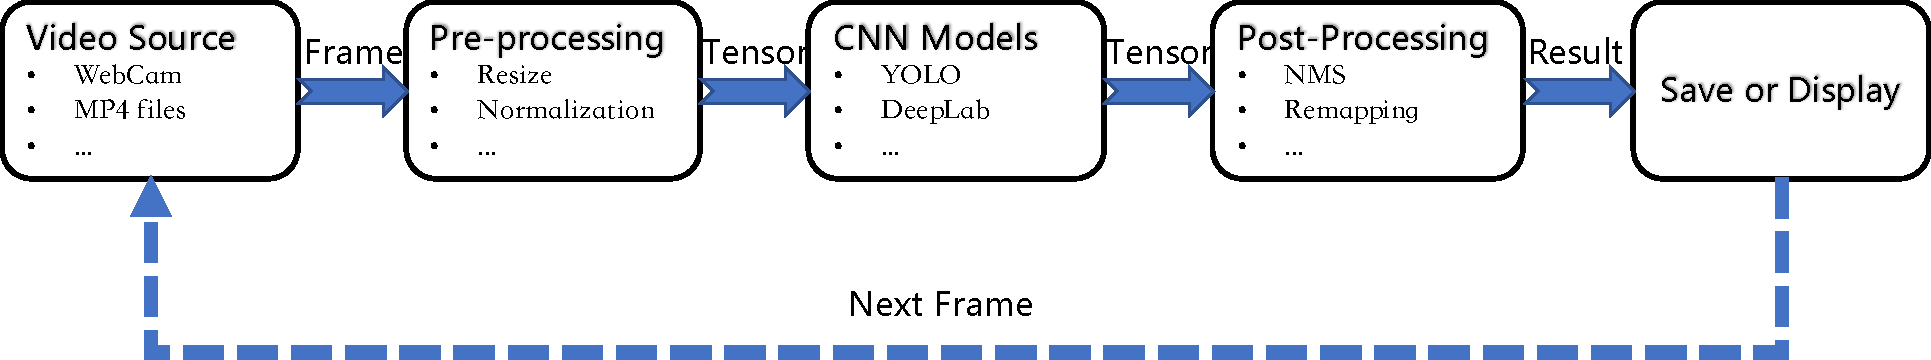
\includegraphics[width=\textwidth]{figure/video_proc_flow.pdf}
    \bicaption{深度学习下视频流处理的一般流程}{Genral process of deep learning based video processing workflow}
    \label{fig:video_proc_flow}
\end{figure}
在深度学习技术的背景下,这些视频分析任务虽然会使用到不同的机器学习算法的组合,但是也存在着许多共通的处理流程。% (emmm,可以考虑加一个流程示意图)
一般情况下,视频流的处理可以看作是在连续的视频帧上做单张图像的视觉计算。因此,视频处理通常由视频流的读取,视频帧的预处理,视觉算法模型(CNN)的运行,算法推理结果的后处理,以及结果的输出与展示这几部分共同来构成,如图\ref{fig:video_proc_flow}所示。当然,对于具体的现实任务来说每一个处理步骤中可能还存在一系列的子步骤,最终会使得整个处理流程的可视化表示变成一个较为复杂的有向无环图(Directed Acyclic Graph,DAG)\footnote{这里不考虑如图\ref{fig:video_proc_flow}中前后帧之间的连接。}。 本文接下来要讨论的视频流处理的优化工作也是基于对视频处理的这种理解与抽象。\par

\section{视频流处理的优化策略}\label{intro_opt}
在\ref{intro_vp}中讨论的视频流处理过程可以进行多层面的优化。从底层硬件到系统运行框架再到算法层面,都有着相应的优化工作。一些相关优化工作也会在第\ref{related_work}章做进一步的讨论。因此本部分仅对相关优化策略做简单介绍:\par

\subsection{针对整体处理流程的系统优化。}\label{sub:sys_opt}
对于像图\ref{fig:video_proc_flow}所示的视频处理过程,由于其存在多阶、相互依赖的连续数据处理的特点,视频处理算法的部署可以参考现代CPU流水线式的处理逻辑,通过多级流水线的模式来部分掩藏处理流程中瓶颈模块的计算耗时。另一方面,对于较复杂DAG连接的视频处理任务,其任务本身就存在一定的并行度,可同时对多个模块并行处理。
\subsection{针对视频特性的视觉算法优化}\label{sub:algo_opt}
现有的深度学习视频分析处理算法多数是直接对视频中的每一帧单独运行原本应用在图像上的视觉算法模型,较少考虑视频帧与帧之间连贯性的特点做算法上的专门优化,从而减少算法在处理过程中的冗余或者非必要计算。在利用视频信息的连贯性上,可引入视频光流估计方法,将前帧的计算结果更快速地传递给后一帧,如Zhu et al.提出的DFF(Deep Feature Flow)模型\cite{zhu2017deep};也可以利用视频编码如H.264\cite{tourapis2003fast}中包含的运动向量(Motion Vector)信息,来对视频关键帧进行选择性检测与传播,如Mao et al.提出的MobiEye\cite{mao2019mobieye};
还可以单纯利用短时间内物体的位移量较小的特点,直接利用上一帧的检测结果,进行接下来的细粒度检测,如Google 的人手追踪模型\cite{mediapipe_hand}。此外,也可利用视频帧的上下文信息来提升视频单帧的检测精度\cite{zhu2017flow}。
\subsection{针对神经网络推理的加速优化}\label{sub:infer_opt}
整个深度学习视频处理流程中的速度瓶颈往往是在神经网络模型的推理步骤上,如\ref{intro_dl}中所说,深度神经网络的推理通常需要进行大量的矩阵计算,有数倍于传统计算处理步骤的时间开销。因此在近年来关于神经网络的压缩,剪枝,量化的研究收到了极大的关注。这些技术从不同的角度对深度神经网络模型精简,在保持模型精度的条件下,尽可能减少模型所需计算资源,提升模型运行速度。此外也有专门针对神经网络推理运算的系统层面的优化加速,比如对需要推理的网络模型进行重编译,对满足特定条件的计算步骤进行融合,从而降低相应算子的调用开销,并优化内存空间的使用。

\subsection{针对模型计算特性的硬件优化}\label{sub:HW_opt}
日渐成熟的深度学习算法的使用也促进了相关硬件平台的发展。深度神经网络所需要进行的矩阵运算对并行计算有着天然的适应性。各大厂商生产的GPU,TPU,VPU等异构芯片在处理这类简单多数据计算时相比传统CPU芯片有着明显的优势。Nvidia在近年来着重发展其GPU产品的AI计算能力,在Volta架构后,为其GPU添加了专门的Tensor Core计算核心来提高其在大量矩阵运算上的处理性能;Google在TPU\cite{jouppi2017datacenter}(Tensor Processing Unit)架构中引入了由大量矩阵乘加器构成的脉动阵列(Systolic Array)结构,来提高矩阵运算的吞吐量;Intel也有推出其集成DSP,VLIW,GPU等特性的混合架构VPU\cite{moloney2014myriad}(Vision Processing Unit),来为移动或边缘设备提供视觉相关AI加速计算的能力。\par~\par

本研究期望对具有一般性的基于深度学习的视频处理任务进行部署与性能上的优化,并通过一种通用框架的形式实现。基于这样的研究目标,我们提出了Accel-Video Pipe (简称AVPipe)这一针对智能视频流处理的编程框架。我们在接下来的框架设计与优化的过程中会主要关注\ref{sub:sys_opt}中介绍的视频流处理在系统层面的优化,同时我们的框架会对现有的神经网络推理优化引擎(\ref{sub:infer_opt})以及相应的计算硬件(\ref{sub:HW_opt})提供充分的支持。对于\ref{sub:algo_opt}中的算法层面优化,由于这类有较强的任务相关性,缺少通用性,故在本框架中不做深入,但用户仍可以通过AVPipe实现相应处理任务的算法优化。

\section{论文的主要内容与章节安排}
本论文大致分为五章展开。在接下来的第二章中,我们将对与本文介绍的视频处理相关的已有优化工作进行介绍,并在其中说明现有相关工作的不足以及可借鉴之处。然后在第三章中,我们将总结现有深度学习相关视频处理任务在实际生产应用中的应用需求以及可能存在的问题,并依此来明确我们的研究动机以及研究目标。
在第四章中,我们将详细介绍我们提出并实现的视频流处理编程框架Accel-Video Pipe,这其中包括AVPipe框架的设计逻辑,主体结构,以及它的自动化部署与优化工具。最后,在第五章中,我们将通过几个示例视频项目的开发,以及性能分析对比,来说明本框架在实际应用过程中的有效性。